\documentclass{article}
\usepackage{pdfpages}

\usepackage[english]{babel}
% \usepackage[utf8]{inputenc}
\usepackage{inputenc}
\usepackage{url}

\usepackage{hyperref}
\graphicspath{ {images/final/} }

\usepackage[nottoc]{tocbibind}

% Latex commands / macros
    \newcommand{\mat}[2][ccccccccccccccccccccccccccccccccccccccccccccc]
	    {\left[ \arraycolsep=4pt\def\arraystretch{1.5}
				\begin{array}{#1} #2 \\ 
				\end{array} 
		\right]}

	\newcommand{\crossmat}[1]{\mat{#1{^X}}}

	\newcommand{\pvec}[1]{\vec{#1}\mkern2mu\vphantom{#1}}

    % Position vector macros
    \newcommand{\pspr}{\pvec{p}'_s} % position of the tool sphere (display)
    \newcommand{\ps}{\pvec{p}_s} % position of the tool rear (inertial)

    \newcommand{\prpr}{\pvec{p}'_r} % position of the tool rear (display)
    \newcommand{\pr}{\pvec{p}_r} % position of the tool rear (inertial)

    \newcommand{\pfpr}{\pvec{p}'_f}
    \newcommand{\pf}{\pvec{p}_f}

    \newcommand{\pc}{\pvec{p}_c}
    \newcommand{\pd}{\pvec{p}_d}

    % Attitude macros
    \newcommand{\Ad}{\mathbf{A}_d} % attitude of the display
    \newcommand{\Ac}{\mathbf{A}_c} % attitude of the camera
    \newcommand{\At}{\mathbf{A}_t} % attitude of the tool
    \newcommand{\Atpr}{\mathbf{A}'_t} % attitude of the tool

    \newcommand{\Adinv}{\mathbf{A}^{-1}_d} % attitude of the display
    \newcommand{\Acinv}{\mathbf{A}^{-1}_c} % attitude of the camera
    \newcommand{\Atinv}{\mathbf{A}^{-1}_t} % attitude of the tool

    % Quaternion macros
	\newcommand{\q}{\overline{\mathbf{q}}}
	\newcommand{\dq}{\overline{\delta \vec{q}}}
	\newcommand{\qc}{\q_c}
	\newcommand{\qd}{\q_d}
	\newcommand{\qt}{\q_t}

	% Covariance matrix macros
	\newcommand{\Pac}{\mathbf{P}_{ac}}
	\newcommand{\Pad}{\mathbf{P}_{ad}}
	\newcommand{\Pat}{\mathbf{P}_{at}}

	\newcommand{\Pacpr}{\mathbf{P}'_{ac}}
	\newcommand{\Padpr}{\mathbf{P}'_{ad}}
	\newcommand{\Patpr}{\mathbf{P}'_{at}}

	\newcommand{\Pps}{\mathbf{P}_{ps}}
	\newcommand{\Ppr}{\mathbf{P}_{pr}}
	\newcommand{\Ppf}{\mathbf{P}_{pf}}
	\newcommand{\Ppc}{\mathbf{P}_{pc}}
	\newcommand{\Ppd}{\mathbf{P}_{pd}}

	\newcommand{\Ppspr}{\mathbf{P}'_{ps}}
	\newcommand{\Pprpr}{\mathbf{P}'_{pr}}
	\newcommand{\Ppfpr}{\mathbf{P}'_{pf}}

	\newcommand{\el}{\vec{l}}




%%%%%%%%%%%%%%%%%%%%%%%%%%%%%%%%%%%%%%%%%%%%%%%%%%%%%%%%%%%%%%%%%%%%%%%%%%%%%%%
%% TITLE PAGE
%%%%%%%%%%%%%%%%%%%%%%%%%%%%%%%%%%%%%%%%%%%%%%%%%%%%%%%%%%%%%%%%%%%%%%%%%%%%%%%

\begin{document}
% https://en.wikibooks.org/wiki/LaTeX/Title_Creation
% \begin{titlepage}

	\title{The 3D Interaction Tool: A Pointing Device for Virtual Reality Applications}
	\author{Lukas Gemar}
	\date{March 26, 2016}
	\maketitle

% \end{titlepage}


%%%%%%%%%%%%%%%%%%%%%%%%%%%%%%%%%%%%%%%%%%%%%%%%%%%%%%%%%%%%%%%%%%%%%%%%%%%%%%%
%% START DOCUMENT
%%%%%%%%%%%%%%%%%%%%%%%%%%%%%%%%%%%%%%%%%%%%%%%%%%%%%%%%%%%%%%%%%%%%%%%%%%%%%%%

\begin{abstract}
The 3D Interaction Tool is a hand-held device that enables a user to interact with virtual reality applications. Since both the position and orientation of the tool are tracked, user input with the tool accomplishes tasks such as selecting, translating, and rotating three-dimensional objects, or free-hand drawing in space. The tool�s position is tracked by a software application that filters observations from a camera attached to the virtual reality display, and the orientation is found by means of observations from an inertial measurement unit attached to the tool itself. Simple computer-aided design and drawing applications demonstrate the capabilities of the 3D Interaction Tool. 
\end{abstract}

\begin{flushleft}

\section{Nomenclature}

% Position vector definitions
\textbf{Position vectors definitions in the inertial coordinate frame}: \\
$ \ps \equiv $ position of the spherical tracking target on tool rear \\
$ \pr \equiv $ position of the tool rear \\
$ \pf \equiv $ position of the tool front \\
$ \pc \equiv $ position of the tracking camera \\
$ \pd \equiv $ position of the virtual reality display \\

\medskip

% Rotated position vector definitions
\textbf{Rotated position vectors}: \\
$ \pspr \equiv $ position of the spherical tracking target on tool rear, camera coordinates \\
$ \prpr \equiv $ position of the tool rear in display coordinates \\
$ \pfpr \equiv $ position of the tool front in display coordinates \\

\medskip

% Attitude matrix definitions
\textbf{Attitude matrices}: \\
$ \Ac \equiv $ attitude of the tracking camera \\
$ \Ad \equiv $ attitude of the virtual reality display \\
$ \At \equiv $ attitude of the interaction tool \\
$ \Atpr \equiv $ attitude of the interaction tool in display coordinates \\

\medskip

% Quaternion definitions
\textbf{Body-referenced quaternion representations of attitude}: \\
$ \qc \equiv $ attitude of the tracking camera \\
$ \qd \equiv $ attitude of the virtual reality display \\
$ \qt \equiv $ attitude of the interaction tool \\

\medskip

% Covariance definitions
\textbf{Position error covariances in inertial coordinate frame}: \\
$ \Pps \equiv $ covariance of spherical tracking target position \\
$ \Ppr \equiv $ covariance of the position of the rear of the interaction tool\\
$ \Ppf \equiv $ covariance of the position of the front of the interaction tool\\
$ \Ppc \equiv $ covariance of the position of the tracking camera \\
$ \Ppd \equiv $ covariance of the position of the virtual reality display \\

\medskip

\textbf{Attitude error covariances in the inertial coordinate frame}: \\
$ \Pac \equiv $ covariance of the tracking camera attitude quaternion error \\
$ \Pad \equiv $ covariance of the display attitude quaternion error \\
$ \Pat \equiv $ covariance of the interaction tool attitude quaternion error \\

\medskip

\textbf{Position error covariances in rotated body coordinates}: \\
$ \Ppspr \equiv $ covariance of the sphereical tracking target position \\
$ \Pprpr \equiv $ covariance of the position of the rear of the interaction tool \\
$ \Ppfpr \equiv $ covariance of the position of the front of the interaction tool \\

\medskip

\textbf{Attitude error covariances in the rotated body coordinates}: \\
$ \Pacpr \equiv $ covariance of the tracking camera attitude angular error \\
$ \Padpr \equiv $ covariance of the display attitude angular error \\
$ \Patpr \equiv $ covariance of the interaction tool attitude angular error \\

\section{Introduction}

\subsection{Motivation: Direct input for VR}

As much as \$25 billion could be spent on virtual reality (VR) and augmented reality (AR) software applications by 2025 \cite{Bloomberg-01-13}. There are two primary modes of user-input that are possible for these applications: indirect and direct. Indirect input devices translate the user's physical movements into the motion of a virtual cursor by means of a fixed transformation. Common examples of indirect input devices are a mouse or joystick. Direct input devices also translate physical to virtual movements, but this transformation is one-to-one. For example, a touch screen is a direct input device because the physical location of the user's press is colocated with the virtual click. 

\medskip

With the advent of virtual reality applications the following question must be answered: which of these input paradigms -- indirect or direct -- will prove most useful for interacting with virtual reality applications? While indirect input devices have achieved widespread popularity for two-dimensional displays, the direct input paradigm for VR applications embraces the immersiveness of VR experiences by enabling intuitive interactions for users. Direct input devices allow users to reach out and interact with the objects of their virtual space, just as they would with objects in their physical space. 

\subsection{Requirements: 12 DOF device tracking}

In order to enable direct input with the interaction tool, the tool's tracking system must estimate both the position and orientation of the interaction tool. Additionally, rendering a virtual representation of the tool requires measuring its position and orientation relative to the virtual reality display orientation, given by the attitude matrix $\Ad$. To track the tool's absolute trajectory, its position is determined relative to the world -- that is, relative to a non-accelerating, inertial coordinate system in the user's physical environment. The position and orientation of the tool in the world coordinates of the inertial frame are $\pf$ and $\At$, respectively. The position of the tool in the coordinate frame of the virtual reality display is denoted by a 'prime' sign: the tip or front of the tool in display coordinates is $\pfpr$. Thus, there are four tracking targets: $\pf$, $\At$, $\pfpr$, and $\Ad$; these are shown in Figure \ref{fig:requirements}. 

\begin{figure}
	\begin{center}
		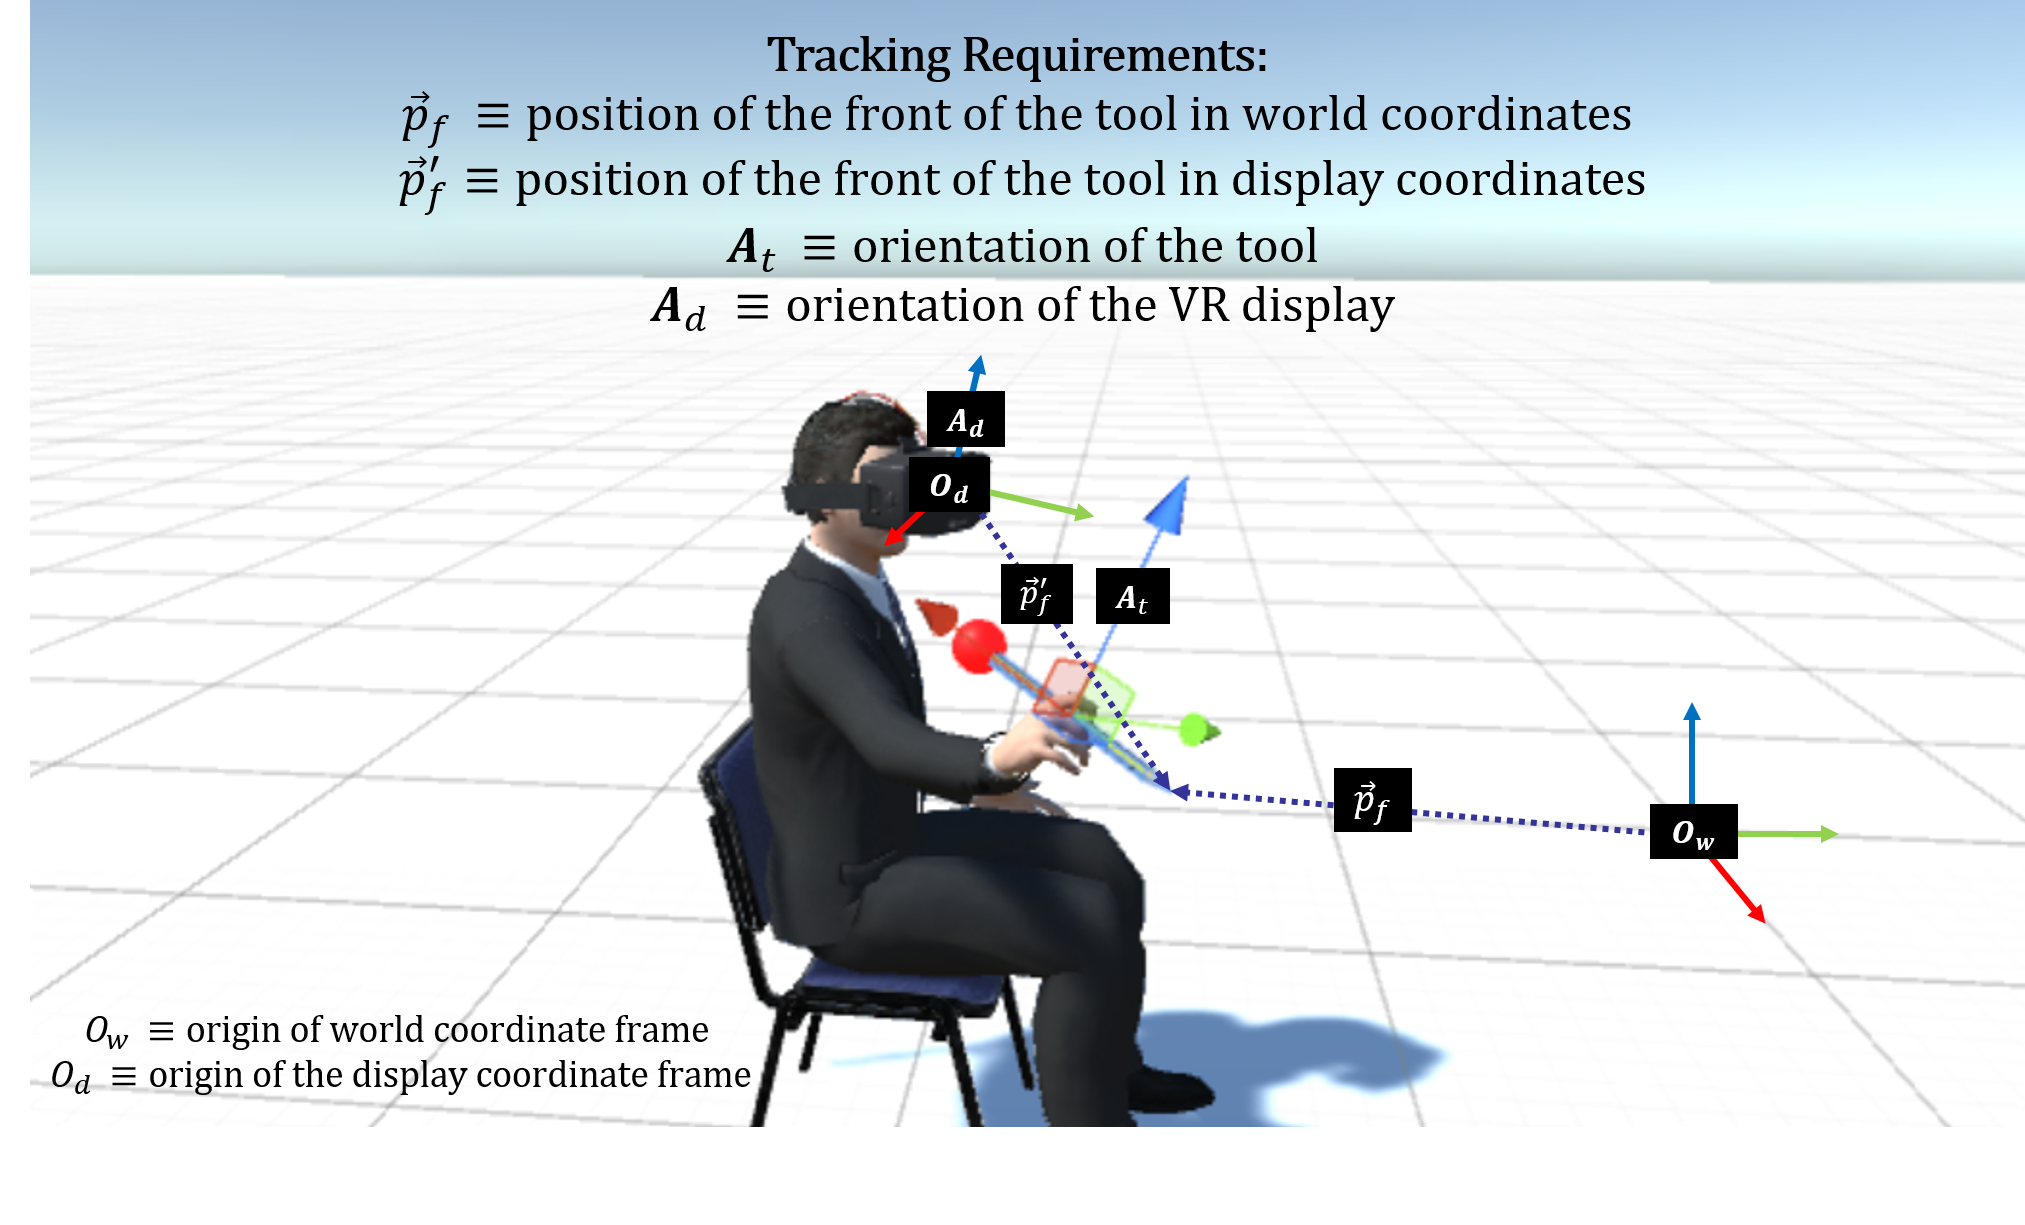
\includegraphics[width=1\textwidth]{requirements}
	\end{center}
	\caption{Position and orientation tracking requirements}
	\label{fig:requirements}
\end{figure}


\subsection{Background}

\subsection{Objectives: Tool usability}

The usability requirements presented in Figure \ref{fig:usability} must be met for the tool to succeed as an \textit{input} device for VR software applications.

\begin{figure}
	\begin{center}
		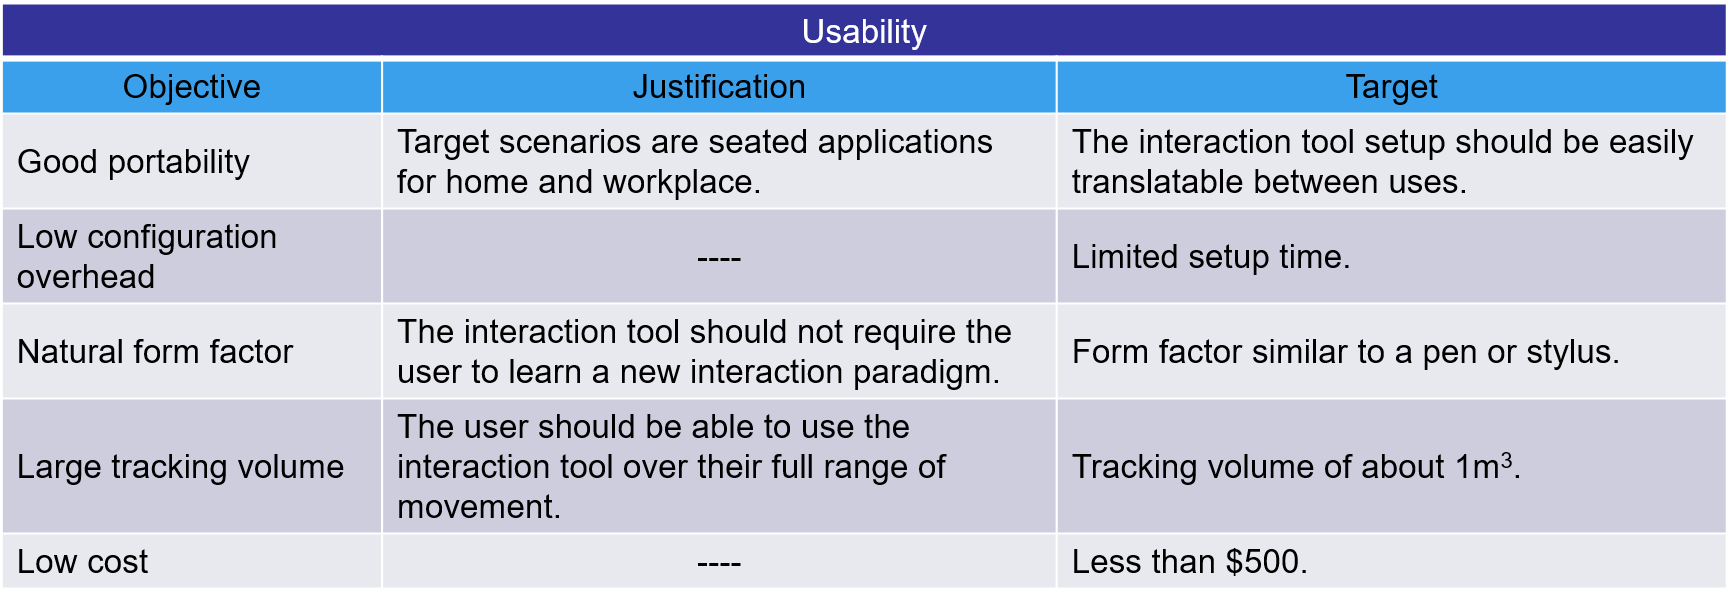
\includegraphics[width=1\textwidth]{Usability}
	\end{center}
	\caption{Usability design objectives}
	\label{fig:usability}
\end{figure}

\subsection{Objectives: Tool tracking performance}

The performance requirements presented in Figure \ref{fig:performance} must be met for the tool to succeed as a \textit{direct} input device for VR software applications.

\begin{figure}
	\begin{center}
		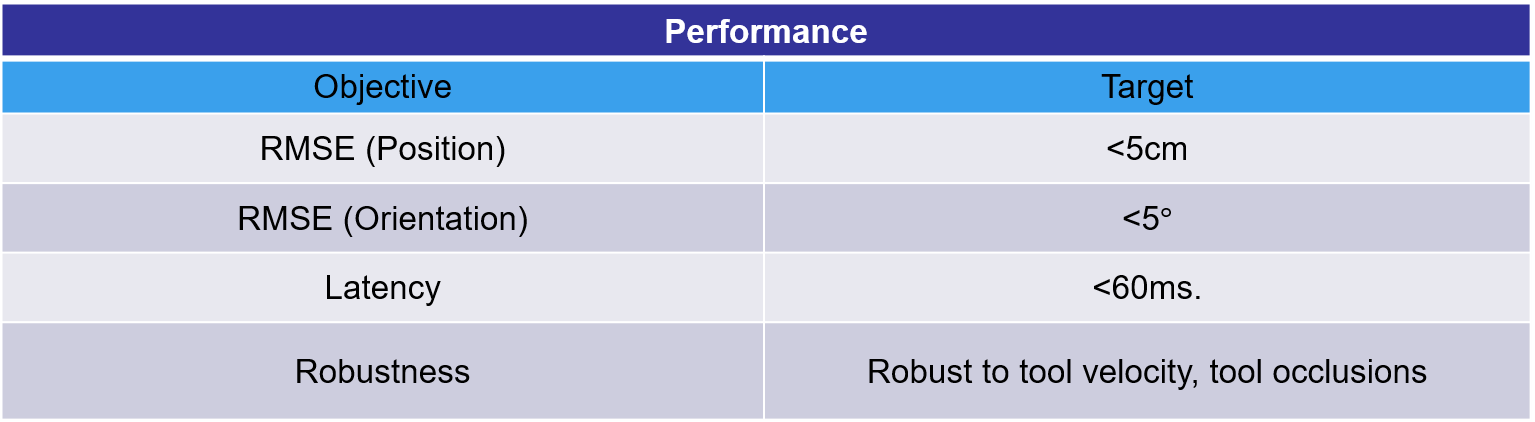
\includegraphics[width=1\textwidth]{Performance}
	\end{center}
	\caption{Performance design objectives}
	\label{fig:performance}
\end{figure}

\section{Tool Tracking Model}

\subsection{Tracking Geometry 1: World-referenced}

The world-referenced tracking geometry is shown in Figure \ref{fig:worldtopo}.

\begin{figure}
	\begin{center}
		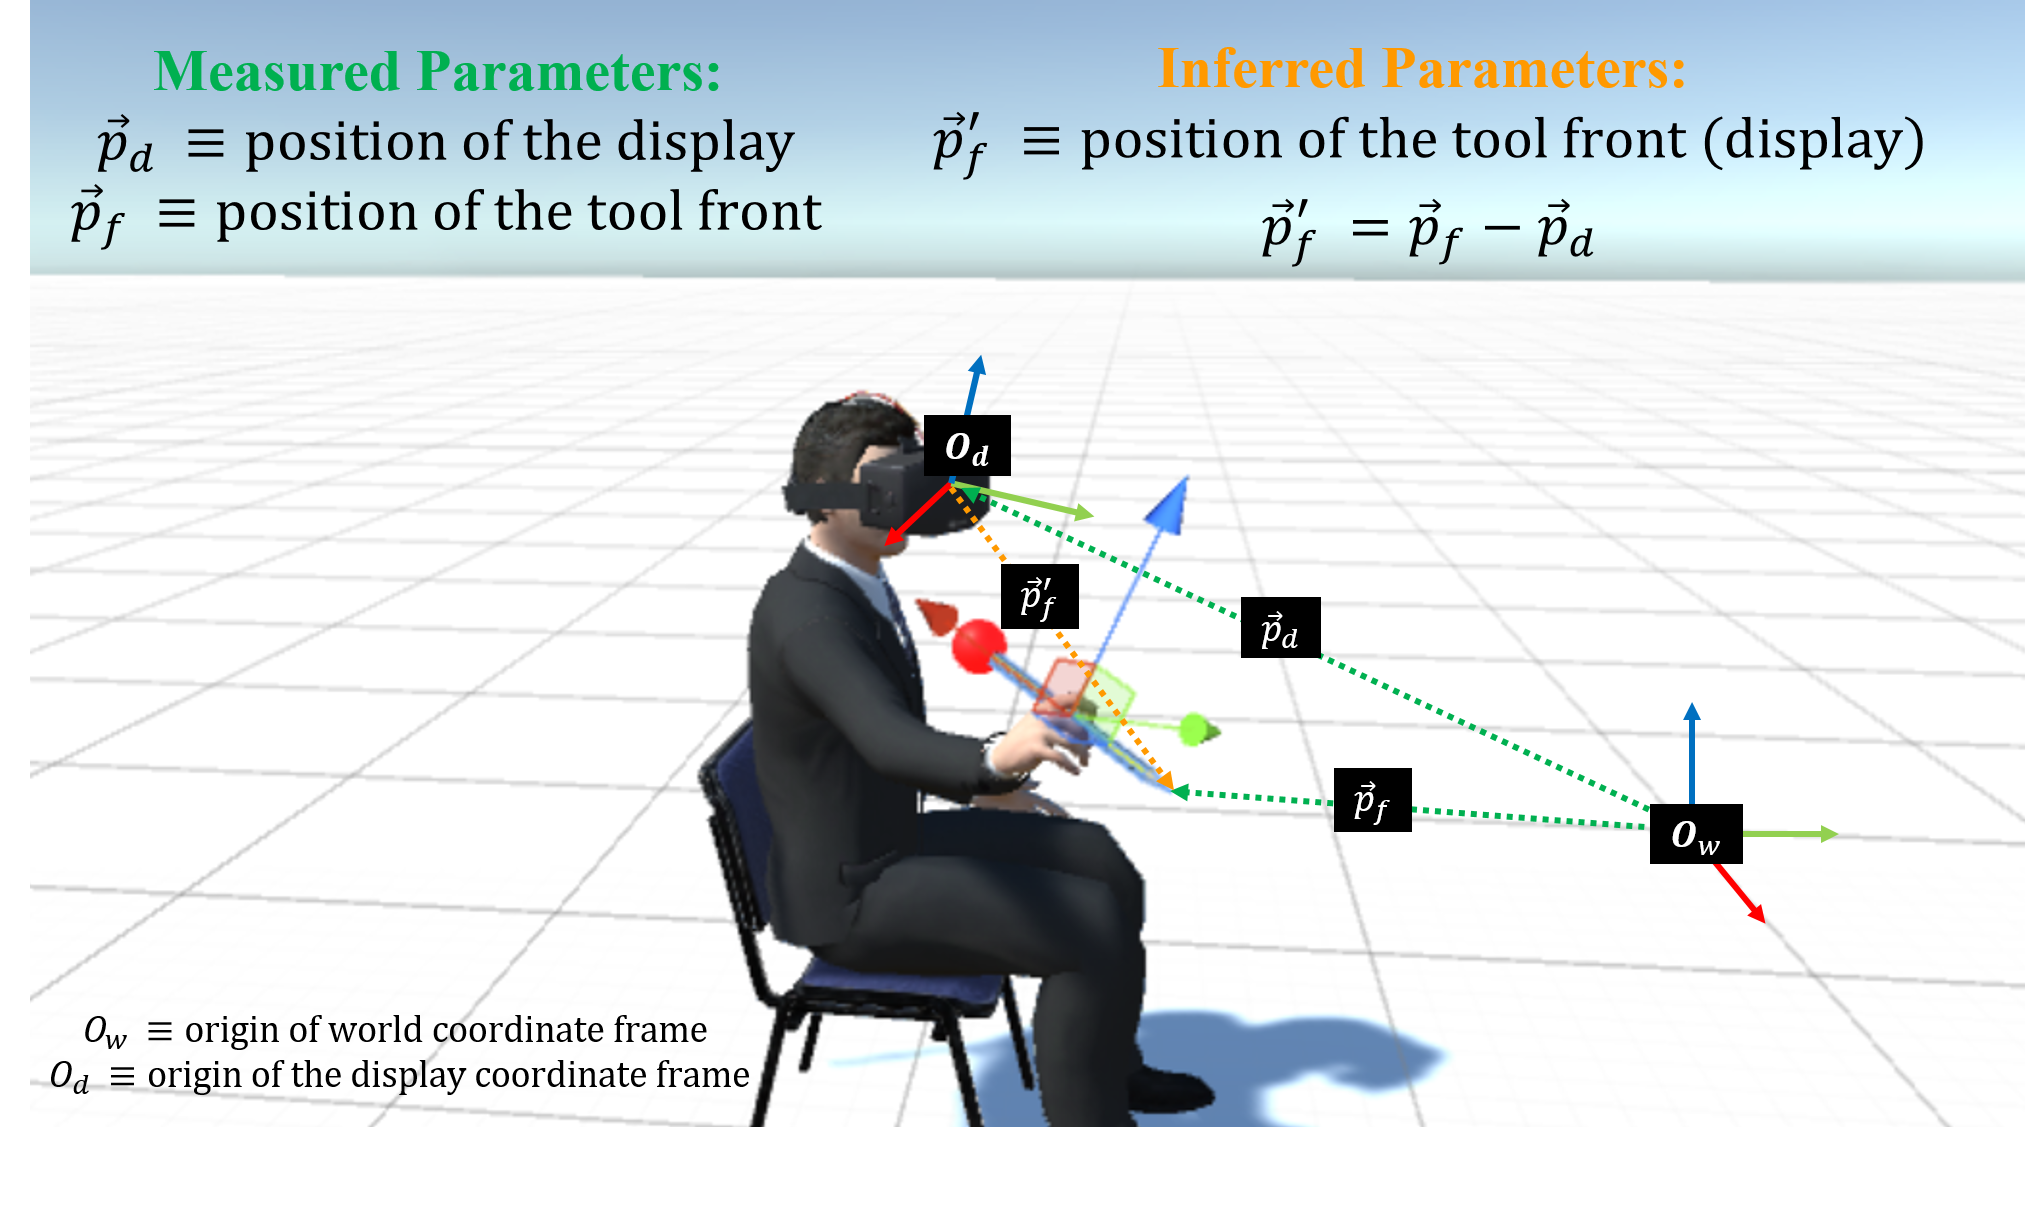
\includegraphics[width=1\textwidth]{WorldTopo}
	\end{center}
	\caption{Position tracking with a world-referenced geometry}
	\label{fig:worldtopo}
\end{figure}

\subsection{Tracking Geometry 2: Display-referenced}

The display-referenced tracking geometry is shown in Figure \ref{fig:displaytopo}.

\begin{figure}
	\begin{center}
		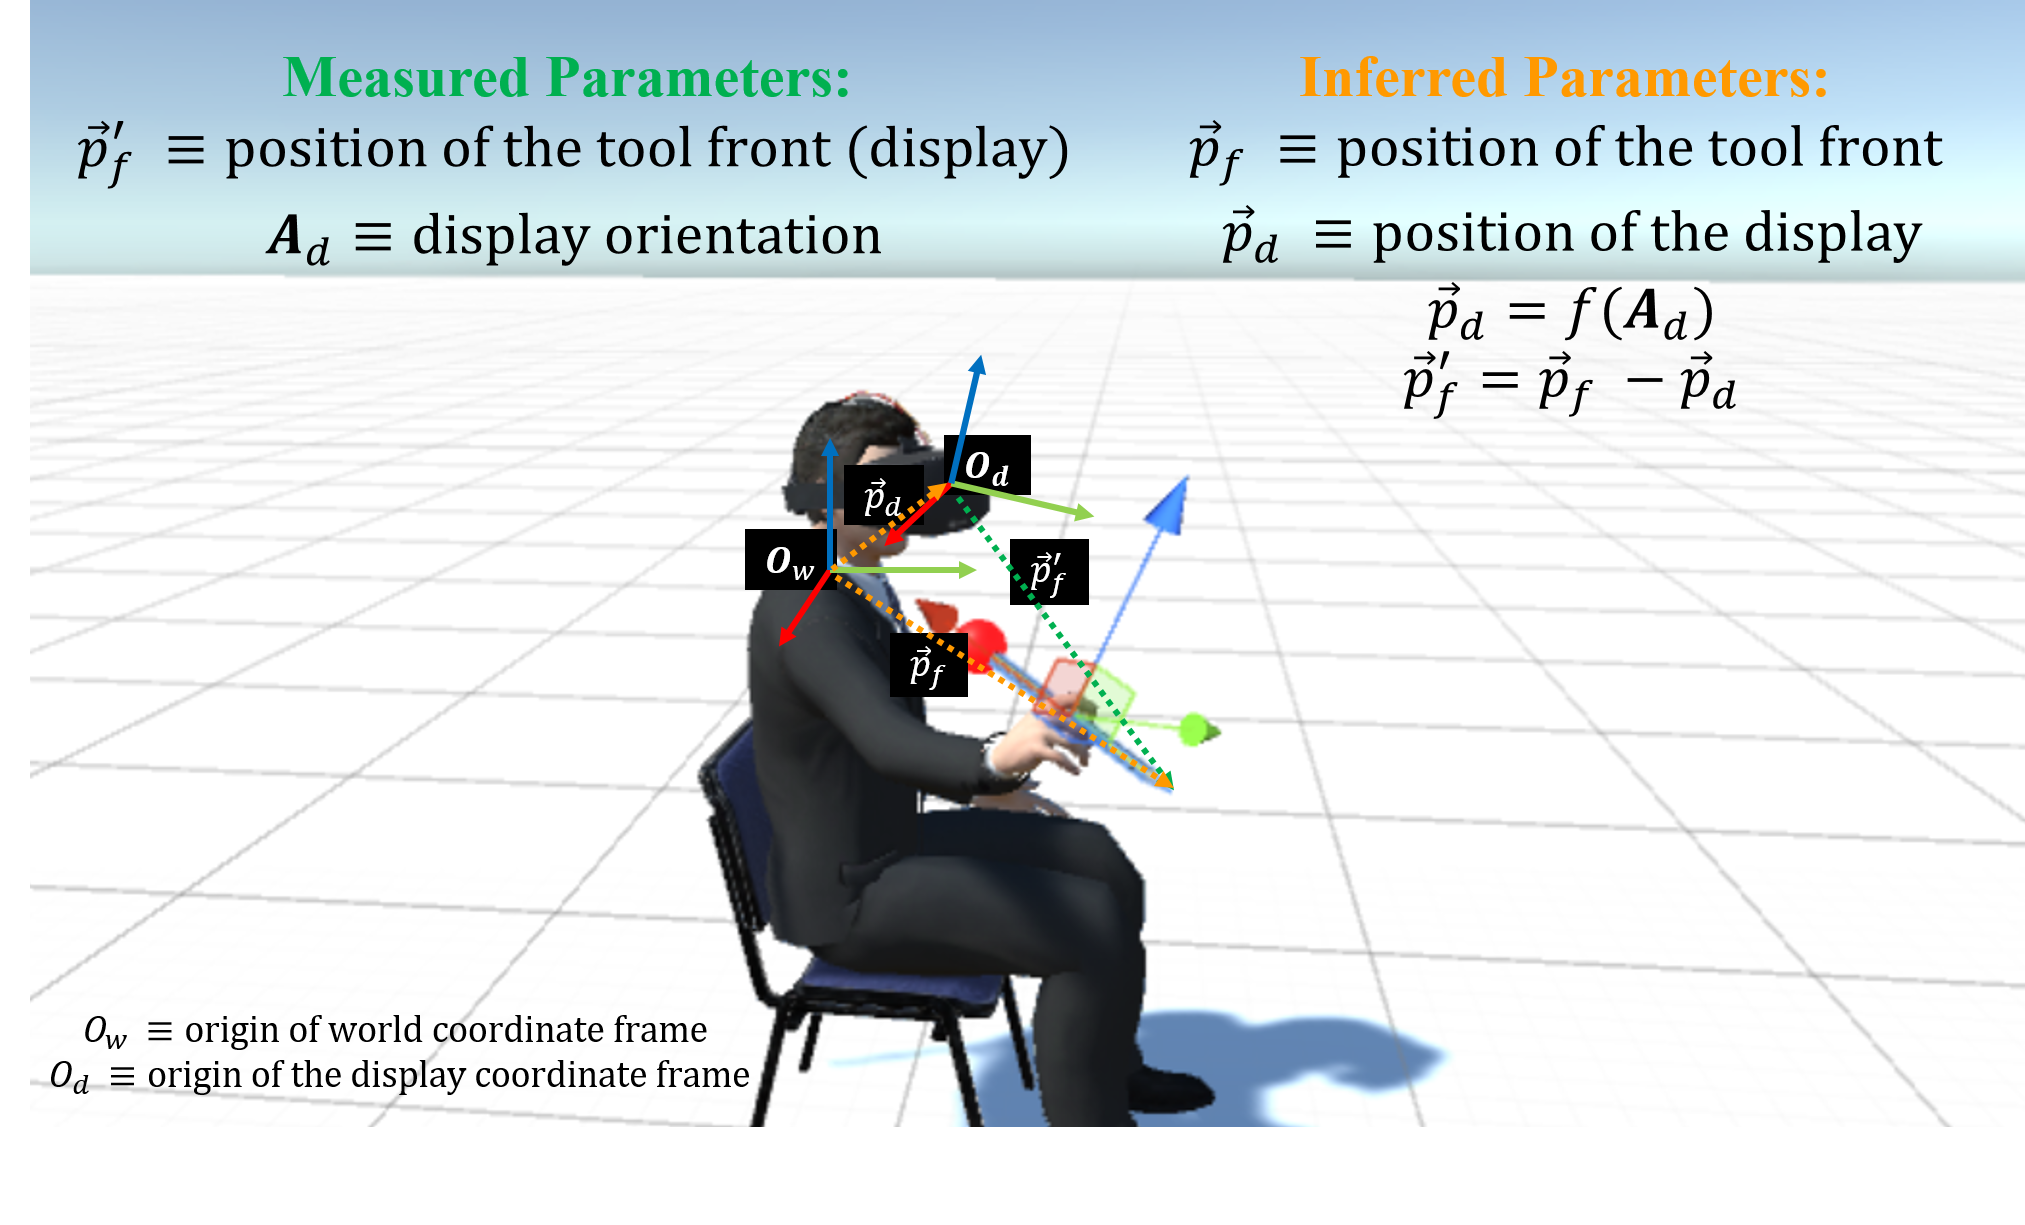
\includegraphics[width=1\textwidth]{DisplayTopo}
	\end{center}
	\caption{Position tracking with a display-referenced geometry}
	\label{fig:displaytopo}
\end{figure}

\subsection{Model Selection: Display-referenced tracking}

\subsection{Tracking measurements}

Not all of these three tracking targets are measured directly. The tracking targets are inferred from the measurements of the position of the rear of the interaction tool relative to the camera, the attitude of the camera, and the attitude of the tool. The position of the tool relative to the camera is denoted by $\pspr$, the attitude of the camera relative to the inertial coordinate system by $\Ac$ and the attitude of the tool relative to the inertial coordinate system by $\At$. The vector $\pspr$ is measured by finding the .

\subsection{Inferring the tool position}

\subsection{Inferring the tool attitude}

% Position and attitude equations
$$ \pr = \Acinv \pspr - \pc $$
$$ \pf = \pr + \Atinv \el $$
$$ \pfpr = \Ad (\pf + \pd) $$
$$ \Atpr = \Ad \Atinv \el $$

% Covariance equations
$$ \Pprpr = \Ppspr + \crossmat{\pspr} \Pacpr \crossmat{\pspr}^T $$
$$ \Ppr = \Acinv ( \Ppspr + \crossmat{\pspr} \Pacpr \crossmat{\pspr}^T ) (\Acinv)^T + \Ppc $$
$$ \Ppf = \Ppr + \Atinv \crossmat{\el} \Patpr \crossmat{\el}^T (\Atinv)^T $$
$$ \Ppfpr = \Ad ( \Ppf + \Ppd ) \Ad{^T} $$
$$ \Ppfpr = \Ppspr + \crossmat{\pspr} \Pacpr \crossmat{\pspr}^T + \Atpr \crossmat{\el} \Patpr \crossmat{\el}^T (\Atpr)^T + 2\Ad\Ppd\Ad{^T} $$
        



\bibliographystyle{ieeetr}
\bibliography{references}

\end{flushleft}
\end{document} 
